\documentclass[twoside]{book}

% Packages required by doxygen
\usepackage{calc}
\usepackage{doxygen}
\usepackage{graphicx}
\usepackage[utf8]{inputenc}
\usepackage{makeidx}
\usepackage{multicol}
\usepackage{multirow}
\usepackage{textcomp}
\usepackage[table]{xcolor}

% Font selection
\usepackage[T1]{fontenc}
\usepackage{mathptmx}
\usepackage[scaled=.90]{helvet}
\usepackage{courier}
\usepackage{amssymb}
\usepackage{sectsty}
\renewcommand{\familydefault}{\sfdefault}
\allsectionsfont{%
  \fontseries{bc}\selectfont%
  \color{darkgray}%
}
\renewcommand{\DoxyLabelFont}{%
  \fontseries{bc}\selectfont%
  \color{darkgray}%
}

% Page & text layout
\usepackage{geometry}
\geometry{%
  a4paper,%
  top=2.5cm,%
  bottom=2.5cm,%
  left=2.5cm,%
  right=2.5cm%
}
\tolerance=750
\hfuzz=15pt
\hbadness=750
\setlength{\emergencystretch}{15pt}
\setlength{\parindent}{0cm}
\setlength{\parskip}{0.2cm}
\makeatletter
\renewcommand{\paragraph}{%
  \@startsection{paragraph}{4}{0ex}{-1.0ex}{1.0ex}{%
    \normalfont\normalsize\bfseries\SS@parafont%
  }%
}
\renewcommand{\subparagraph}{%
  \@startsection{subparagraph}{5}{0ex}{-1.0ex}{1.0ex}{%
    \normalfont\normalsize\bfseries\SS@subparafont%
  }%
}
\makeatother

% Headers & footers
\usepackage{fancyhdr}
\pagestyle{fancyplain}
\fancyhead[LE]{\fancyplain{}{\bfseries\thepage}}
\fancyhead[CE]{\fancyplain{}{}}
\fancyhead[RE]{\fancyplain{}{\bfseries\leftmark}}
\fancyhead[LO]{\fancyplain{}{\bfseries\rightmark}}
\fancyhead[CO]{\fancyplain{}{}}
\fancyhead[RO]{\fancyplain{}{\bfseries\thepage}}
\fancyfoot[LE]{\fancyplain{}{}}
\fancyfoot[CE]{\fancyplain{}{}}
\fancyfoot[RE]{\fancyplain{}{\bfseries\scriptsize Generated on Sun Jan 14 2018 19\-:16\-:27 for A\-V\-L Tree by Doxygen }}
\fancyfoot[LO]{\fancyplain{}{\bfseries\scriptsize Generated on Sun Jan 14 2018 19\-:16\-:27 for A\-V\-L Tree by Doxygen }}
\fancyfoot[CO]{\fancyplain{}{}}
\fancyfoot[RO]{\fancyplain{}{}}
\renewcommand{\footrulewidth}{0.4pt}
\renewcommand{\chaptermark}[1]{%
  \markboth{#1}{}%
}
\renewcommand{\sectionmark}[1]{%
  \markright{\thesection\ #1}%
}

% Indices & bibliography
\usepackage{natbib}
\usepackage[titles]{tocloft}
\setcounter{tocdepth}{3}
\setcounter{secnumdepth}{5}
\makeindex

% Hyperlinks (required, but should be loaded last)
\usepackage{ifpdf}
\ifpdf
  \usepackage[pdftex,pagebackref=true]{hyperref}
\else
  \usepackage[ps2pdf,pagebackref=true]{hyperref}
\fi
\hypersetup{%
  colorlinks=true,%
  linkcolor=blue,%
  citecolor=blue,%
  unicode%
}

% Custom commands
\newcommand{\clearemptydoublepage}{%
  \newpage{\pagestyle{empty}\cleardoublepage}%
}


%===== C O N T E N T S =====

\begin{document}

% Titlepage & ToC
\hypersetup{pageanchor=false}
\pagenumbering{roman}
\begin{titlepage}
\vspace*{7cm}
\begin{center}%
{\Large A\-V\-L Tree }\\
\vspace*{1cm}
{\large Generated by Doxygen 1.8.6}\\
\vspace*{0.5cm}
{\small Sun Jan 14 2018 19:16:27}\\
\end{center}
\end{titlepage}
\clearemptydoublepage
\tableofcontents
\clearemptydoublepage
\pagenumbering{arabic}
\hypersetup{pageanchor=true}

%--- Begin generated contents ---
\chapter{Class Index}
\section{Class List}
Here are the classes, structs, unions and interfaces with brief descriptions\-:\begin{DoxyCompactList}
\item\contentsline{section}{\hyperlink{classAVLTree}{A\-V\-L\-Tree} }{\pageref{classAVLTree}}{}
\end{DoxyCompactList}

\chapter{File Index}
\section{File List}
Here is a list of all files with brief descriptions\-:\begin{DoxyCompactList}
\item\contentsline{section}{/home/travis/build/ob-\/algdati-\/ws17/blatt-\/7-\/aufgabe-\/1-\/sbem/avltree/\hyperlink{AVLTree_8cpp}{A\-V\-L\-Tree.\-cpp} }{\pageref{AVLTree_8cpp}}{}
\item\contentsline{section}{/home/travis/build/ob-\/algdati-\/ws17/blatt-\/7-\/aufgabe-\/1-\/sbem/avltree/\hyperlink{AVLTree_8h}{A\-V\-L\-Tree.\-h} \\*This header file contains all required definitions and basic utilities to creat and manage self balancing trees (A\-V\-L-\/\-Tree) }{\pageref{AVLTree_8h}}{}
\end{DoxyCompactList}

\chapter{Class Documentation}
\hypertarget{classAVLTree}{\section{A\-V\-L\-Tree Class Reference}
\label{classAVLTree}\index{A\-V\-L\-Tree@{A\-V\-L\-Tree}}
}


{\ttfamily \#include $<$A\-V\-L\-Tree.\-h$>$}

\subsection*{Public Member Functions}
\begin{DoxyCompactItemize}
\item 
\hyperlink{classAVLTree_af4a1d1be1b6301ba59c6e101c6efc6ba}{$\sim$\-A\-V\-L\-Tree} ()
\item 
Node $\ast$ \hyperlink{classAVLTree_a03178f48ba61b538ec0b1394fec938b4}{search} (const int)
\begin{DoxyCompactList}\small\item\em Searching fo a node with specified value. \end{DoxyCompactList}\item 
void \hyperlink{classAVLTree_a50bc0809a20d87d79838b98b30e94ece}{insert} (const int)
\begin{DoxyCompactList}\small\item\em Adding a node with specified value to the tree. \end{DoxyCompactList}\item 
void \hyperlink{classAVLTree_a8671295418947911e9387549116f89eb}{remove} (const int)
\begin{DoxyCompactList}\small\item\em Removing the node with specified key, if exists. \end{DoxyCompactList}\item 
vector$<$ int $>$ $\ast$ \hyperlink{classAVLTree_a2a9e456d5db8167232a4b3bfca987abf}{preorder} () const 
\item 
vector$<$ int $>$ $\ast$ \hyperlink{classAVLTree_aeadd0a31d0366168b5e2accc04f2f481}{inorder} () const 
\item 
vector$<$ int $>$ $\ast$ \hyperlink{classAVLTree_a953fe7b7d3bce08e8d266db544c03415}{postorder} () const 
\end{DoxyCompactItemize}
\subsection*{Friends}
\begin{DoxyCompactItemize}
\item 
ostream \& \hyperlink{classAVLTree_a1c2fe2fa878a3a4e7c2315ac417b2721}{operator$<$$<$} (ostream \&, const \hyperlink{classAVLTree}{A\-V\-L\-Tree} \&)
\end{DoxyCompactItemize}


\subsection{Detailed Description}
The \hyperlink{classAVLTree}{A\-V\-L\-Tree} class represents the self balancing tree (A\-V\-L-\/\-Tree) 

\subsection{Constructor \& Destructor Documentation}
\hypertarget{classAVLTree_af4a1d1be1b6301ba59c6e101c6efc6ba}{\index{A\-V\-L\-Tree@{A\-V\-L\-Tree}!$\sim$\-A\-V\-L\-Tree@{$\sim$\-A\-V\-L\-Tree}}
\index{$\sim$\-A\-V\-L\-Tree@{$\sim$\-A\-V\-L\-Tree}!AVLTree@{A\-V\-L\-Tree}}
\subsubsection[{$\sim$\-A\-V\-L\-Tree}]{\setlength{\rightskip}{0pt plus 5cm}A\-V\-L\-Tree\-::$\sim$\-A\-V\-L\-Tree (
\begin{DoxyParamCaption}
{}
\end{DoxyParamCaption}
)}}\label{classAVLTree_af4a1d1be1b6301ba59c6e101c6efc6ba}
Default destructor of \hyperlink{classAVLTree}{A\-V\-L\-Tree}. 

\subsection{Member Function Documentation}
\hypertarget{classAVLTree_aeadd0a31d0366168b5e2accc04f2f481}{\index{A\-V\-L\-Tree@{A\-V\-L\-Tree}!inorder@{inorder}}
\index{inorder@{inorder}!AVLTree@{A\-V\-L\-Tree}}
\subsubsection[{inorder}]{\setlength{\rightskip}{0pt plus 5cm}vector$<$ int $>$ $\ast$ A\-V\-L\-Tree\-::inorder (
\begin{DoxyParamCaption}
{}
\end{DoxyParamCaption}
) const}}\label{classAVLTree_aeadd0a31d0366168b5e2accc04f2f481}
\hypertarget{classAVLTree_a50bc0809a20d87d79838b98b30e94ece}{\index{A\-V\-L\-Tree@{A\-V\-L\-Tree}!insert@{insert}}
\index{insert@{insert}!AVLTree@{A\-V\-L\-Tree}}
\subsubsection[{insert}]{\setlength{\rightskip}{0pt plus 5cm}void A\-V\-L\-Tree\-::insert (
\begin{DoxyParamCaption}
\item[{const int}]{value}
\end{DoxyParamCaption}
)}}\label{classAVLTree_a50bc0809a20d87d79838b98b30e94ece}


Adding a node with specified value to the tree. 

This method adds a node with the given value to the tree, if there is no other node with the same key and balances the tree if required.


\begin{DoxyParams}{Parameters}
{\em Key} & the key of the node to be added to the tree. \\
\hline
\end{DoxyParams}
\hypertarget{classAVLTree_a953fe7b7d3bce08e8d266db544c03415}{\index{A\-V\-L\-Tree@{A\-V\-L\-Tree}!postorder@{postorder}}
\index{postorder@{postorder}!AVLTree@{A\-V\-L\-Tree}}
\subsubsection[{postorder}]{\setlength{\rightskip}{0pt plus 5cm}vector$<$ int $>$ $\ast$ A\-V\-L\-Tree\-::postorder (
\begin{DoxyParamCaption}
{}
\end{DoxyParamCaption}
) const}}\label{classAVLTree_a953fe7b7d3bce08e8d266db544c03415}
\hypertarget{classAVLTree_a2a9e456d5db8167232a4b3bfca987abf}{\index{A\-V\-L\-Tree@{A\-V\-L\-Tree}!preorder@{preorder}}
\index{preorder@{preorder}!AVLTree@{A\-V\-L\-Tree}}
\subsubsection[{preorder}]{\setlength{\rightskip}{0pt plus 5cm}vector$<$ int $>$ $\ast$ A\-V\-L\-Tree\-::preorder (
\begin{DoxyParamCaption}
{}
\end{DoxyParamCaption}
) const}}\label{classAVLTree_a2a9e456d5db8167232a4b3bfca987abf}
\hypertarget{classAVLTree_a8671295418947911e9387549116f89eb}{\index{A\-V\-L\-Tree@{A\-V\-L\-Tree}!remove@{remove}}
\index{remove@{remove}!AVLTree@{A\-V\-L\-Tree}}
\subsubsection[{remove}]{\setlength{\rightskip}{0pt plus 5cm}void A\-V\-L\-Tree\-::remove (
\begin{DoxyParamCaption}
\item[{const int}]{key}
\end{DoxyParamCaption}
)}}\label{classAVLTree_a8671295418947911e9387549116f89eb}


Removing the node with specified key, if exists. 

This method removes a node with the given value as key, if there is a node with the same value.


\begin{DoxyParams}{Parameters}
{\em Key} & the key of the node to be removed from the tree. \\
\hline
\end{DoxyParams}
\hypertarget{classAVLTree_a03178f48ba61b538ec0b1394fec938b4}{\index{A\-V\-L\-Tree@{A\-V\-L\-Tree}!search@{search}}
\index{search@{search}!AVLTree@{A\-V\-L\-Tree}}
\subsubsection[{search}]{\setlength{\rightskip}{0pt plus 5cm}A\-V\-L\-Tree\-::\-Node $\ast$ A\-V\-L\-Tree\-::search (
\begin{DoxyParamCaption}
\item[{const int}]{value}
\end{DoxyParamCaption}
)}}\label{classAVLTree_a03178f48ba61b538ec0b1394fec938b4}


Searching fo a node with specified value. 

This method searches for a node with a specified key. returns the node with the value if it is found or nullprt if not found.


\begin{DoxyParams}{Parameters}
{\em Key} & the value to be searched for. \\
\hline
\end{DoxyParams}
\begin{DoxyReturn}{Returns}
Node the node with value as key if exists or nullptr otherwise. 
\end{DoxyReturn}


\subsection{Friends And Related Function Documentation}
\hypertarget{classAVLTree_a1c2fe2fa878a3a4e7c2315ac417b2721}{\index{A\-V\-L\-Tree@{A\-V\-L\-Tree}!operator$<$$<$@{operator$<$$<$}}
\index{operator$<$$<$@{operator$<$$<$}!AVLTree@{A\-V\-L\-Tree}}
\subsubsection[{operator$<$$<$}]{\setlength{\rightskip}{0pt plus 5cm}ostream\& operator$<$$<$ (
\begin{DoxyParamCaption}
\item[{ostream \&}]{, }
\item[{const {\bf A\-V\-L\-Tree} \&}]{}
\end{DoxyParamCaption}
)\hspace{0.3cm}{\ttfamily [friend]}}}\label{classAVLTree_a1c2fe2fa878a3a4e7c2315ac417b2721}


The documentation for this class was generated from the following files\-:\begin{DoxyCompactItemize}
\item 
/home/travis/build/ob-\/algdati-\/ws17/blatt-\/7-\/aufgabe-\/1-\/sbem/avltree/\hyperlink{AVLTree_8h}{A\-V\-L\-Tree.\-h}\item 
/home/travis/build/ob-\/algdati-\/ws17/blatt-\/7-\/aufgabe-\/1-\/sbem/avltree/\hyperlink{AVLTree_8cpp}{A\-V\-L\-Tree.\-cpp}\end{DoxyCompactItemize}

\chapter{File Documentation}
\hypertarget{AVLTree_8cpp}{\section{/home/travis/build/ob-\/algdati-\/ws17/blatt-\/7-\/aufgabe-\/1-\/sbem/avltree/\-A\-V\-L\-Tree.cpp File Reference}
\label{AVLTree_8cpp}\index{/home/travis/build/ob-\/algdati-\/ws17/blatt-\/7-\/aufgabe-\/1-\/sbem/avltree/\-A\-V\-L\-Tree.\-cpp@{/home/travis/build/ob-\/algdati-\/ws17/blatt-\/7-\/aufgabe-\/1-\/sbem/avltree/\-A\-V\-L\-Tree.\-cpp}}
}
{\ttfamily \#include $<$functional$>$}\\*
{\ttfamily \#include \char`\"{}A\-V\-L\-Tree.\-h\char`\"{}}\\*
Include dependency graph for A\-V\-L\-Tree.\-cpp\-:
\nopagebreak
\begin{figure}[H]
\begin{center}
\leavevmode
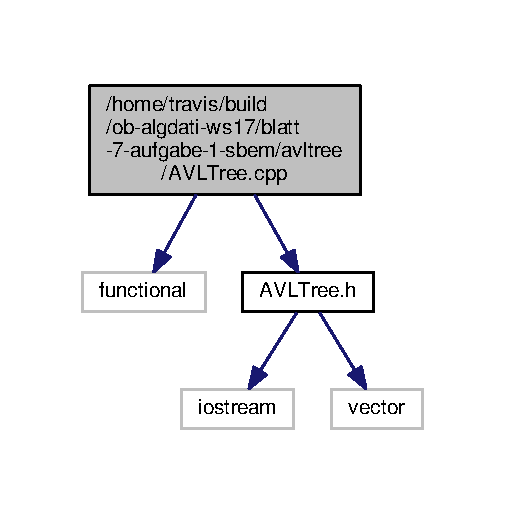
\includegraphics[width=243pt]{AVLTree_8cpp__incl}
\end{center}
\end{figure}
\subsection*{Functions}
\begin{DoxyCompactItemize}
\item 
std\-::ostream \& \hyperlink{AVLTree_8cpp_af27b8a8e936a7ebca0f1febcde35e381}{operator$<$$<$} (std\-::ostream \&os, const \hyperlink{classAVLTree}{A\-V\-L\-Tree} \&tree)
\end{DoxyCompactItemize}


\subsection{Function Documentation}
\hypertarget{AVLTree_8cpp_af27b8a8e936a7ebca0f1febcde35e381}{\index{A\-V\-L\-Tree.\-cpp@{A\-V\-L\-Tree.\-cpp}!operator$<$$<$@{operator$<$$<$}}
\index{operator$<$$<$@{operator$<$$<$}!AVLTree.cpp@{A\-V\-L\-Tree.\-cpp}}
\subsubsection[{operator$<$$<$}]{\setlength{\rightskip}{0pt plus 5cm}std\-::ostream\& operator$<$$<$ (
\begin{DoxyParamCaption}
\item[{std\-::ostream \&}]{os, }
\item[{const {\bf A\-V\-L\-Tree} \&}]{tree}
\end{DoxyParamCaption}
)}}\label{AVLTree_8cpp_af27b8a8e936a7ebca0f1febcde35e381}

\hypertarget{AVLTree_8h}{\section{/home/travis/build/ob-\/algdati-\/ws17/blatt-\/7-\/aufgabe-\/1-\/sbem/avltree/\-A\-V\-L\-Tree.h File Reference}
\label{AVLTree_8h}\index{/home/travis/build/ob-\/algdati-\/ws17/blatt-\/7-\/aufgabe-\/1-\/sbem/avltree/\-A\-V\-L\-Tree.\-h@{/home/travis/build/ob-\/algdati-\/ws17/blatt-\/7-\/aufgabe-\/1-\/sbem/avltree/\-A\-V\-L\-Tree.\-h}}
}


This header file contains all required definitions and basic utilities to creat and manage self balancing trees (A\-V\-L-\/\-Tree).  


{\ttfamily \#include $<$iostream$>$}\\*
{\ttfamily \#include $<$vector$>$}\\*
Include dependency graph for A\-V\-L\-Tree.\-h\-:
\nopagebreak
\begin{figure}[H]
\begin{center}
\leavevmode
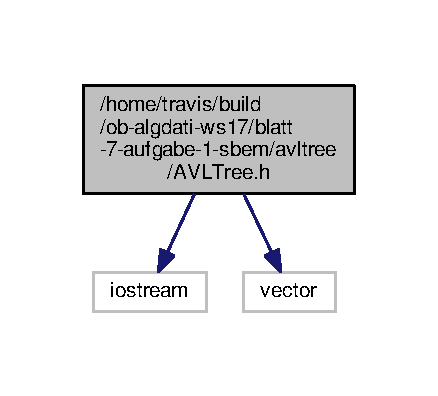
\includegraphics[width=210pt]{AVLTree_8h__incl}
\end{center}
\end{figure}
This graph shows which files directly or indirectly include this file\-:
\nopagebreak
\begin{figure}[H]
\begin{center}
\leavevmode
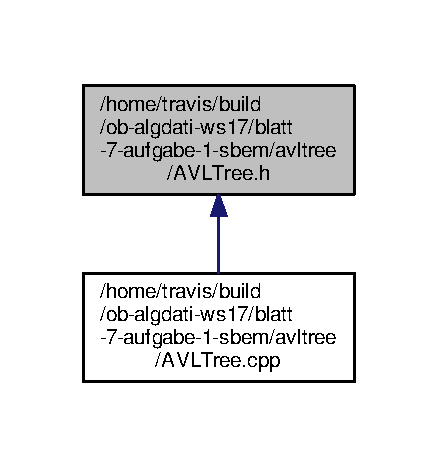
\includegraphics[width=210pt]{AVLTree_8h__dep__incl}
\end{center}
\end{figure}
\subsection*{Classes}
\begin{DoxyCompactItemize}
\item 
class \hyperlink{classAVLTree}{A\-V\-L\-Tree}
\end{DoxyCompactItemize}


\subsection{Detailed Description}
This header file contains all required definitions and basic utilities to creat and manage self balancing trees (A\-V\-L-\/\-Tree). \begin{DoxyAuthor}{Authors}
Ehsan Moslehi, Sebastian Bauman 
\end{DoxyAuthor}
\begin{DoxyVersion}{Version}
1.\-1 This Library contains all required definitions and basic utilities to creat and manage self balancing trees (A\-V\-L-\/\-Tree). Use folowing methods to manage A\-V\-L-\/\-Tree insert to add nodes to the tree remove to remove nodes from the tree search to search a node 
\end{DoxyVersion}

%--- End generated contents ---

% Index
\newpage
\phantomsection
\addcontentsline{toc}{chapter}{Index}
\printindex

\end{document}
